%amsart class
\documentclass[a4paper, 10pt, reqno]{amsart}

%Packages
\usepackage[utf8]{inputenc}
\usepackage[english]{babel}
\usepackage{graphics}
\usepackage{physics}
\usepackage{listings}
\usepackage{hyperref}
\usepackage{blindtext}
\usepackage{xcolor}
\usepackage[position=top]{subfig}
\usepackage{pgf}
\usepackage{tikz}
\usepackage{tikzscale}
\usepackage{pgfplots}
\usepackage{placeins}
\usepackage{parskip}

\hypersetup{colorlinks=true, linkcolor=black, citecolor=black,
urlcolor=blue}
%\hypersetup{hidelinks}

\pgfplotsset{compat=1.5}
\newlength\figureheight
\newlength\figurewidth
\setlength\figurewidth{0.98\textwidth}
\setlength\figureheight{0.75\figurewidth}

\usepackage{etoolbox}
\makeatletter
\patchcmd{\@maketitle}
  {\ifx\@empty\@dedicatory}
  {\ifx\@empty\@date \else {\vskip3ex
  \centering\footnotesize\@date\par\vskip1ex}\fi
   \ifx\@empty\@dedicatory}
  {}{}
\patchcmd{\@adminfootnotes}
  {\ifx\@empty\@date\else \@footnotetext{\@setdate}\fi}
  {}{}{}
\makeatother

%Custom colors
\definecolor{code}{rgb}{0.9, 0.17, 0.31}
\definecolor{coolgrey}{rgb}{0.55, 0.57, 0.67}
\definecolor{cyan(process)}{rgb}{0.0, 0.72, 0.92}
\definecolor{lightwhite}{rgb}{0.9647058823529412, 0.9647058823529412, 0.9647058823529412}
\definecolor{royalblue}{rgb}{0.25, 0.41, 0.88}
\definecolor{mediumseagreen}{rgb}{0.24, 0.7, 0.44}
%listing customization
\lstset{ %
  backgroundcolor=\color{lightwhite},
  basicstyle=\ttfamily\footnotesize,        % the size of the fonts that are used for the code
  breakatwhitespace=true,         % sets if automatic breaks should only happen at whitespace
  breaklines=true,                 % sets automatic line breaking
  captionpos=b,                    % sets the caption-position to bottom
  commentstyle=\color{mediumseagreen},    % comment style
  deletekeywords={...},            % if you want to delete keywords from the given language
  escapeinside={\%*}{*)},          % if you want to add LaTeX within your code
  extendedchars=true,              % lets you use non-ASCII characters; for 8-bits encodings only, does not work with UTF-8
  frame=single,	                   % adds a frame around the code
  keepspaces=true,                 % keeps spaces in text, useful for keeping indentation of code (possibly needs columns=flexible)
  keywordstyle=\color{code},       % keyword style
  language=[90]Fortran,                 % the language of the code
  otherkeywords={...},           % if you want to add more keywords to the set
  emph={get_H_p, spline, exp, abs, sqrt},
  emphstyle={\color{royalblue}},
  rulecolor=\color{white},         % if not set, the frame-color may be changed on line-breaks within not-black text (e.g. comments (green here))
  numbers=left,
  showspaces=false,                % show spaces everywhere adding particular underscores; it overrides 'showstringspaces'
  showstringspaces=false,          % underline spaces within strings only
  showtabs=false,                  % show tabs within strings adding particular underscores
  stepnumber=1,                    % the step between two line-numbers. If it's 1, each line will be numbered
  tabsize=3,	                   % sets default tabsize to 2 spaces
}

%Frontpage stuff
\title[Milestone 1]{\Large{Milestone 2: The recombination history of the universe} \\
\normalsize{AST5220 - Cosmology 2}}

\author[San]{Metin San}

\date{\today}



%Begining document
\begin{document}

\maketitle
\begin{center}
   \vspace*{-0.6cm} \textsc{\url{https://github.com/MetinSa/AST5220/tree/master/milestone2}}
\end{center}

\begin{abstract}
We compute the free electron fraction, $X_e$,  which describes the ionization history of the Universe. This is done through the use of the Saha equation for $X_e \geq 0.99$, while the Peebles equation is used for $X_e < 0.99$. We then apply $X_e$ to acquire the electron number density $n_e$, which in turn is used to compute the optical depth $\tau$ and the visibility function $g$. The resulting $\tau$ and $g$ indicate that recombination occurred around $z \approx 1100$.
\end{abstract}

\section{Introduction}
This is the second milestone on the path to simulating the Cosmic Microwave
Background (CMB). The goal of this milestone will be to study the
recombination history of the Universe. Our main objectives will be to
calculate the optical depth and the visibility function of the Universe. These
quantities are needed for the coming milestones where we are to integrate the
Boltzmann-Einstein equations. We will acquire these by computing the
ionization fraction of hydrogen in the early universe from which both the
optical depth and visibility function can be derived.

Similarly to Milestone 1, the programs used for the numerical calculations are
written in FORTRAN 90 and based on a provided skeleton code. The analysis of
the results are done using Python. The source code and tools used to produce
the following results and figures can be found on my Github by following the
link below the author name on the front page.

The report will consist of a theory section where the relevant physics and
assumptions are motivated and introduced. What follows is a section where we
discuss the numerical implementation and methods used to solve the various
equations. We continue by presenting the results of the study in a results
section. The report is then concluded with a brief conclusion section where we
reflect back on the work done.

\section{Theory}

We assume that the reader is familiar with Milestone 1 and will therefore not
repeat the definitions and equations previously presented. The first quantity
of interest in this milestone is the electron number density, $n_e$. We can
find this through the free electron fraction, which is defined as
\begin{equation}\label{eq: X_e}
    X_{e} \equiv \frac{n_{e}}{n_{\mathrm{H}}}=\frac{n_{e}}{n_{b}}.
\end{equation}
Here $n_{\mathrm{H}}$ is the total number density of hydrogen which we
approximate to be equal to the baryon number density, $n_{\mathrm{b}}$, by
ignoring helium. The hydrogen density is given as 
\begin{equation}\label{eq: n_e}
    n_{\mathrm{H}}=n_{b} \simeq
    \frac{\rho_{b}}{m_{\mathrm{H}}}=\frac{\Omega_{b} \rho_{c}}{m_{\mathrm{H}}
    a^{3}},
\end{equation}
where $\rho_b$ and $\rho_c$ are the baryon and the critical density today,
respectively, and $m_\mathrm{H}$ is the mass of the hydrogen atom.

Prior to recombination, the electron fraction can be approximated by the Saha
equation
\begin{equation}\label{eq: saha}
    \frac{X_{e}^{2}}{1-X_{e}} \simeq \frac{1}{n_{b}}\left(\frac{m_{e} T_{b}}{2
    \pi}\right)^{3 / 2} e^{-\epsilon_{0} / T_{b}}.
\end{equation}
Here, $T_b$ is the baryon temperature, $m_e$ the mass of the electron, and
$\epsilon_0$ the ionization energy of hydrogen. The baryon temperature, $T_b$
is approximated to be equal to that of the photons as they were coupled during
these early times
\begin{equation}\label{eq: T_b}
    T_{b} \simeq T_{r}=\frac{T_{0}}{a}, \quad T_{0}=2.725 \mathrm{K}.
\end{equation}
The Saha equation is a good approximation as long as the system we are
considering is in strong thermodynamic equilibrium (TE). However, during
recombination, photons decouple from baryons resulting in the universe
dropping out of TE. We will therefore have to use the more general form of the
Saha equation, namely the Peebles equation, given as
\begin{equation}\label{eq: peeble}
    \frac{d X_{e}}{d
    x}=\frac{C_{r}\left(T_{b}\right)}{H}\left[\beta\left(T_{b}\right)\left(1-
    X_{e}\right)-n_{\mathrm{H}} \alpha^{(2)}\left(T_{b}\right)
    X_{e}^{2}\right].
\end{equation}
The Peebles equation account for important aspects of particle physics which
result in a more accurate calculation of $X_e$. Here $C_r$, $\beta(T_b)$, and
$\alpha^{(2)}(T_b)$ are substitutions defined as
\begin{align}\label{eq: subs}
    C_{r}\left(T_{b}\right)&=\frac{\Lambda_{2 s \rightarrow 1
    s}+\Lambda_{\alpha}}{\Lambda_{2 s \rightarrow 1
    s}+\Lambda_{\alpha}+\beta^{(2)}\left(T_{b}\right)}, \\
    \Lambda_{2 s \rightarrow 1 s}&=8.227 \mathrm{s}^{-1}, \quad
    \Lambda_{\alpha}=H \frac{\left(3 \epsilon_{0}\right)^{3}}{(8 \pi)^{2} n_{1
    s}},\\
    n_{1 s} &=\left(1-X_{e}\right) n_{H}, \\ \beta^{(2)}\left(T_{b}\right)
    &=\beta\left(T_{b}\right) e^{3 \epsilon_{0} / 4 T_{b}},\\
    \beta\left(T_{b}\right)&=\alpha^{(2)}\left(T_{b}\right)\left(\frac{m_{e}
    T_{b}}{2 \pi}\right)^{3 / 2} e^{-\epsilon_{0} / T_{b}},\\
    \alpha^{(2)}\left(T_{b}\right)&=\frac{64 \pi}{\sqrt{27 \pi}}
    \frac{\alpha^{2}}{m_{e}^{2}} \sqrt{\frac{\epsilon_{0}}{T_{b}}}
    \phi_{2}\left(T_{b}\right),\\
    \phi_{2}\left(T_{b}\right) &\simeq 0.448 \ln \left(\epsilon_{0} /
    T_{b}\right).
\end{align}
It should be noted that the above equations are written in terms of natural
units; one should perform a unit analysis and include the missing units before
implementation these into code.

The electron density is of importance to us as it allows us to calculate the
optical depth of the Universe
\begin{equation}\label{eq: tau}
    \tau(\eta)=\int_{\eta}^{\eta_{0}} n_{e} \sigma_{T} a d \eta^{\prime},
\end{equation}
where $\sigma_T$ is the Thompson cross section, $\eta$ is the conformal time,
and the prime denotes $' = d/dx$. The optical depth can be interpreted as the
probability that a photon scatters of an electron. We can also express the
optical depth in a differential form
\begin{equation}\label{eq: tau'}
    \tau^{\prime}= \frac{d\tau}{dx} = -\frac{n_{e} \sigma_{T} a}{\mathcal{H}},
\end{equation}
which makes it easier to compute $\tau$ numerically.

Once acquired, the optical depth allows us the study the final item of
interest during Milestone 2 which is the visibility function
\begin{align}
g(\eta)&=-\dot{\tau} e^{-\tau(\eta)}=-\mathcal{H} \tau^{\prime}
e^{-\tau(x)}=g(x)\label{eq: g},\\
\tilde{g}(x) &\equiv-\tau^{\prime}
e^{-\tau}=\frac{g(x)}{\mathcal{H}(x)}.\label{eq: g_tilde}
\end{align}
Here $\tilde{g}$ is the scaled visibility function, and  $\dot{\tau} =
d\tau/dt$. The visibility function is normalized as
\begin{equation}
    \int_{0}^{\eta_{0}} g(\eta) d \eta=\int_{-\infty}^{0} \tilde{g}(x) d x=1,
\end{equation}
meaning that it gives us the probability for a given observed photon to have
scattered at conformal time $\eta$. We will use $\tilde{g}$ during our
calculations as we are interested in working with functions of $x$, meaning
that when we reference to the visibility function or $g$, we will imply
equation \eqref{eq: g_tilde}.

\section{Implementation}
The implementation for Milestone 2 consists of completing the
\textbf{rec\_mod.f90} module which considers quantities and calculations
related to recombination.

Similar to milestone 1, the code starts by initializing the relevant
parameters and arrays that are to be used during the calculations. These
include recombination grids for the scale factor $a_\mathrm{rec}$, the
redshift $z_\mathrm{rec}$, and the parameter $x_\mathrm{rec}$. In addition,
arrays are allocated for the electron density, $n_e$, the electron fraction
$X_e$, the optical depth $\tau$, and the visibility function, $g$. We proceed
by filling the grids in a linear manner using initial conditions corresponding
to $a_\mathrm{start} = 1$ and $a_\mathrm{stop} = 10^{-10}$.

With the grids initialized, we move on to calculating the free electron
fraction $X_e$. This is done in a loop which runs over all values of $a$ and
$x$. The loop starts by computing the electron number density seen in equation
\eqref{eq: n_e}. What follows is a logic statement which checks the value of
$X_e$. A value of $X_e \geq 0.99$ corresponds to an early Universe in TE,
meaning that we make use of the Saha equation seen in \eqref{eq: saha}. The
Saha equation is solved for $X_e$ which results in the following quadratic
equation
\begin{equation}\label{eq: quad}
    X_{e,i} = \frac{-\gamma_i \pm \sqrt{\gamma_i^2 + 4\gamma_i}}{2}, \qquad
    \gamma_i = \frac{1}{n_{b,i}}\left(\frac{m_e T_b}{2\pi}\right)^{3/2}
    e^{-\epsilon_0/T_b}
\end{equation}
where the quadratic constants are $a = 1$, $b = c = \gamma$, and $n_{b,i}$ is
the baryon density at a given $a_i \in [a_\mathrm{start}, a_\mathrm{stop}]$.
We have chosen to implement an alternate formulation of the quadratic solution
\begin{equation}\label{eq: quad2}
    X_{e,i} = \frac{2}{1 \pm \sqrt{1 + 4/\gamma_i}}. 
\end{equation}
This expression provides the same roots in addition to being a more stable
solution in the case where $\gamma_i \approx 4$. 

However, if $X_e < 0.99$, we assume that the Universe is out of TE and we use
Peebles' equation \eqref{eq: peeble} instead. This is a first order
differential equation, meaning that we solve it using a similar ODE routine as
in Milestone 1. For this purpose, a subroutine is implemented which computes
the RHS of \eqref{eq: peeble}. This is then fed into the ODE routine to return
$X_e$.

Once we have acquired $X_e$ we can easily compute the electron number density
by solving equation \eqref{eq: X_e} for $n_e$. We proceed by splining log
$n_e$, such that it can be evaluated for arbitrary values of $x$ when
necessary. We spline the logarithm because $n_e$ varies over many orders of
magnitude. This means that we have to remember to exponentiate the results
after interpolating. 

With $n_e$ in our possession, we can now compute the optical depth $\tau$.
This is done by solving equation \eqref{eq: tau'}. We observe that this is
another ordinary differential equation, meaning that we solve it in a similar
manner to Peebles' equation with the use of the ODE solver routine, and a
subroutine which computes the RHS of \eqref{eq: tau'}. It follows from the
definition of the optical depth that $\tau = 0$ today which we use as an
initial condition. We proceed by splining log $\tau$ so that it too can be
interpolated at arbitrary $x$. We also implement the calculations of the first
and second derivatives of the optical depth $\tau'$ and $\tau''$ with the use
of the \textit{spline} and \textit{splint\_deriv}, as these are required to
compute the visibility function $g$, and will be of use to us in the coming
milestones.

The final part of the implementation considers the visibility function. Unlike
the other functions, $g$ is directly solvable using $\tau$ and $\tau'$,
resulting in a easy implementation of equation \eqref{eq: g_tilde}. Similarly
to the case with the optical depth, we will again use the same methods as
before to compute $g'$ and $g''$. These are then properly splined to allow for
arbitrary interpolation.

\section{Results}
The results of the fractional electron density is shown as a function of
redshift in figure \ref{fig: X_e}. This proves as a cosmic ionization history.
We observe that the free electron fraction is 1 prior to some hundred redshift
before recombination (z = 1100). Once recombination occurs, the free electron
fraction rapidly drops. We observe a change in the rate of decrease around $z
= 800$.
\begin{figure}
    \centering
    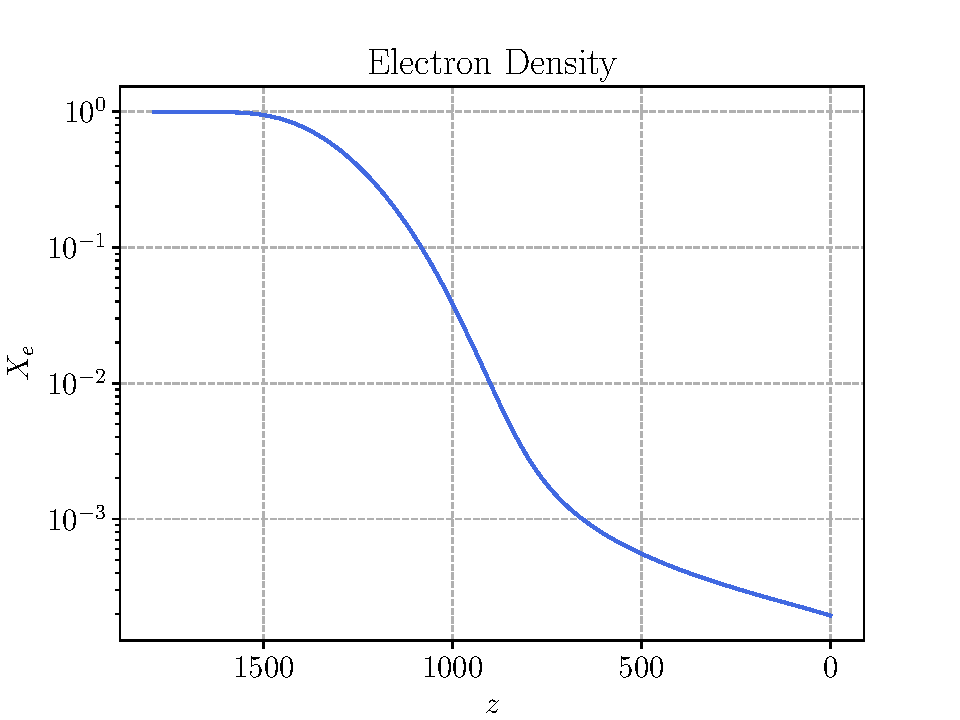
\includegraphics[width = 0.9\textwidth]{xe.pdf}
    \caption{The free electron fraction $X_e$ as a function of redshift $z$.
    The Saha equation \eqref{eq: saha} is used to obtain the values prior to
    $X_e \leq 0.99$ while the Peebles equation \eqref{eq: peeble} is
    integrated to obtain the remaining values}.
    \label{fig: X_e}
\end{figure}

Figure \ref{fig: tau} shows the optical depth of the universe as a function of
$x = \log a$ along with its two derivatives. We observe that the optical depth
closely follows the electron density, as expected from its definition
\eqref{eq: tau}. All three functions are continuous, and closely follow each
other. At $x \approx -7$, corresponding to a redshift of $z \approx 1100$, we
observe $\tau = 1$ which is defined as the boundary between a opaque and
optical thick medium, meaning that the universe became opaque around this
redshift. This coincides well with recombination. The second derivative of the
optical depth experiences a slight increase around $x \approx -7$, likely as a
result of recombination occurring.
\begin{figure}
    \centering
    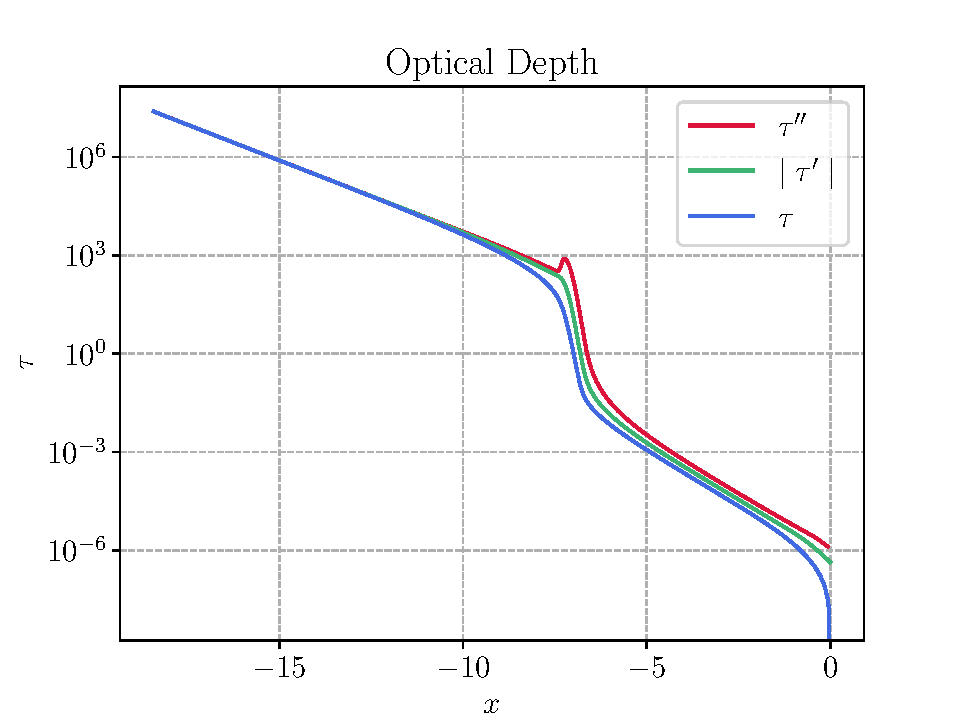
\includegraphics[width = 0.9\textwidth]{tau.pdf}
    \caption{The optical depth $\tau$ along with the first and second
    derivatives $\abs{\tau'}$ and $\tau''$.}
    \label{fig: tau}
\end{figure}

The results of the visibility function calculations are seen in figure
\ref{fig: g}. We have chosen to focus in on the results centered around $x
\approx 7$. Prior to this, the universe was too dense for scattering to occur.
We observe a peak in the visibility function at $x \approx 7$. As mentioned in
the theory section, the visibility function can be interpreted as a
probability distribution of when a CMB photon observed today was last
scattered. These results indicate that this did indeed occur around $ z
\approx 1100$ at the time of recombination.
\begin{figure}
    \centering
    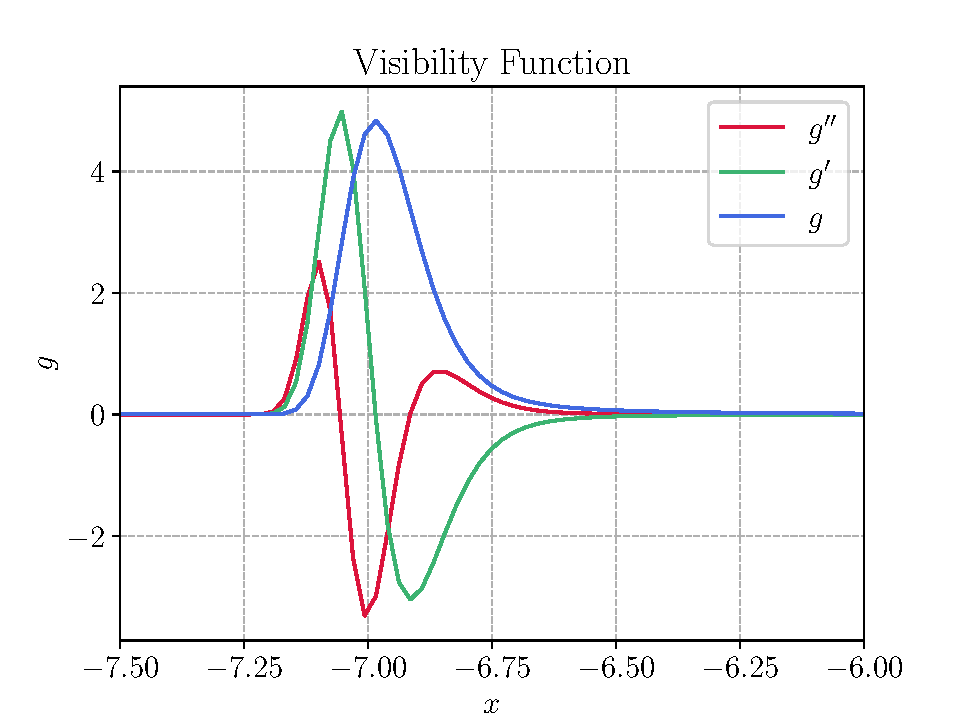
\includegraphics[width = 0.9\textwidth]{g.pdf}
    \caption{The visibility function $g$ along with the first and second
    derivatives $g'/10$ and $g''/300$. The scaling of $g'$ and $g''$ are
    chosen to make the curves fit into the same figure.}
    \label{fig: g}
\end{figure}

\section{Conclusion}
The implementation of Milestone 2 has seemingly been a success. We have
studied the recombination history of the Universe by looking at the ionization
of the Universe through calculating the free electron density. We have then
used these results to study the optical depth of the Universe and the
visibility function. We found that the CMB photons did indeed scatter around
$z \approx 1100$. We are therefore ready to apply these results further to
Milestone 3 where we start considering the evolution of structures in the
Universe.

\nocite{*}
\bibliography{references}{}
\bibliographystyle{plain}
\end{document}